83. Let $\omega_y:\Lambda(x,y)\to\Lambda(x)\otimes\Lambda(y)$ be the algebra homomorphism defined by
\[
\omega_y p_n(x,y)=p_n(x)+(-1)^{n-1}p_n(y). \tag{4}
\]
Equivalently, $\omega_y$ is the automorphism $\omega$ acting on the $y$-variables only. Write $\omega_y f(x,y)=f(x/y)$. In particular, $s_\lambda(x/y)$ is called a \emph{super Schur function}. Let
\[
\Sigma=\operatorname{im}(\omega_y)=\{f(x/y): f\in\Lambda\},
\]
a subalgebra of $\Lambda(x)\otimes\Lambda(y)$.

(e) [3--] Define a \emph{supertableau} of shape $\lambda$ to be an array $T$ of positive integers of shape $\lambda$ such that (i) the rows and columns are weakly increasing, and (ii) the diagonals from the upper left to lower right are strictly increasing (equivalently, there is no $2\times 2$ square of equal entries). A maximal rookwise-connected subset of equal entries is called a \emph{component} of $T$. Let $c(T)$ denote the number of components. For instance, if $T$ is given by:
\begin{center}
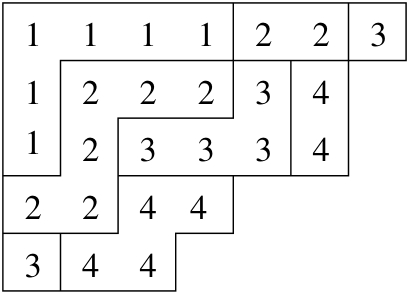
\includegraphics[width=102bp]{figure-original.png}
\end{center}
then $T$ has one component of 1's, two components of 2's, three components of 3's, and two components of 4's, so $c(T)=8$. Show that
\[
s_\lambda(x/x)=\sum_T 2^{c(T)}x^T,
\]
where $T$ ranges over all supertableaux of shape $\lambda$ and $x^T$ has its usual meaning.
